\documentclass[tikz,border=4pt]{standalone}
\usepackage{amsmath}
\begin{document}
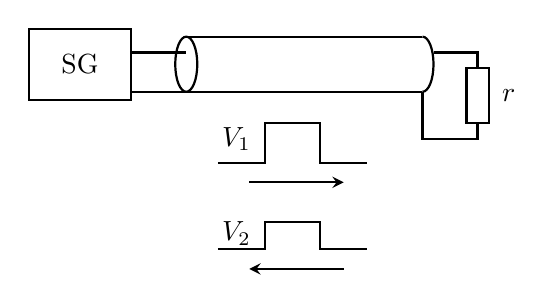
\begin{tikzpicture}[>=stealth, thick, scale=1.0]
  % Signal generator
  \draw[thick] (-1.6, -0.45) rectangle (-0.3, 0.45);
  \node at (-0.95, 0) {SG};

  % Coaxial cable body
  \draw[thick] (0.4, 0.35) -- (3.4, 0.35);
  \draw[thick] (0.4, -0.35) -- (3.4, -0.35);
  \draw[thick] (0.4, 0) ellipse (0.14 and 0.35);
  \draw[thick] (3.4, 0.35) arc (90:-90:0.14 and 0.35);

  % Connections left
  \draw[thick] (-0.3, 0.15) -- (0.4, 0.15);
  \draw[thick] (-0.3, -0.35) -- (0.4, -0.35);

  % Termination resistor r on right
  \draw[thick] (3.54, 0.15) -- (4.1, 0.15) -- (4.1, -0.05);
  \draw[thick] (3.96, -0.05) rectangle (4.24, -0.75);
  \node[right] at (4.28, -0.4) {$r$};
  \draw[thick] (4.1, -0.75) -- (4.1, -0.95) -- (3.4, -0.95) -- (3.4, -0.35);

  % Incident pulse V_1 going right
  \draw[thick] (0.8, -1.25) -- (1.4, -1.25) -- (1.4, -0.75) -- (2.1, -0.75) -- (2.1, -1.25) -- (2.7, -1.25);
  \draw[->] (1.2, -1.50) -- (2.4, -1.50);
  \node[left] at (1.35, -0.95) {$V_1$};

  % Reflected pulse V_2 going left
  \draw[thick] (0.8, -2.35) -- (1.4, -2.35) -- (1.4, -2.00) -- (2.1, -2.00) -- (2.1, -2.35) -- (2.7, -2.35);
  \draw[<-] (1.2, -2.60) -- (2.4, -2.60);
  \node[left] at (1.35, -2.15) {$V_2$};
\end{tikzpicture}
\end{document}
